\documentclass{article}
\usepackage{graphicx,subcaption}
\begin{document}
\section{Supplementary}
\begin{figure*}[th!]
  \centering
  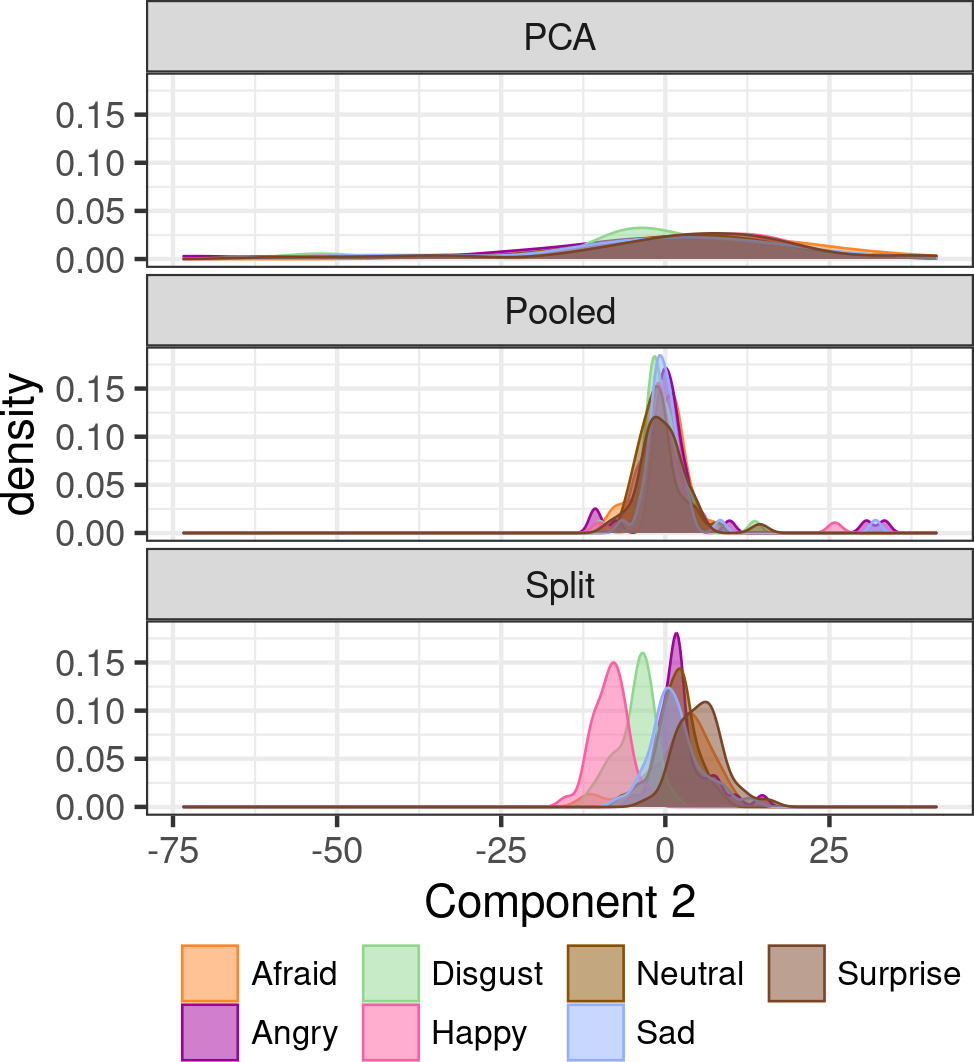
\includegraphics[width = 0.9\textwidth]{figure/PC2_density.png}
  \caption{Density Plots, colored by emotions, of 2nd Component found by PCA, UCA with backgound of all emotional faces except for the afraid emotion pooled (Pooled), and UCA with background of all emotional faces except for the afraid emotion treated separately (Split). This is the same analysis in figure \ref{fig:faces-projected}, except using densities may help readers visualize the difference between pooling and splitting background data.}
  \label{fig:FacesDensity}
\end{figure*}
\end{document}
